%%==================================================
%% chapter01.tex for DUT Thesis 
%% version: 0.1
%% last update: Dec 25th, 2022
%%==================================================




%%%%%%%%%%%%%%%%%%%%%%%%%%%%%%
%
%
%\BiChapter{绪论}{Introduction}
%
%
%
%\BiSection{研究背景与意义}{Research Background}
%
%
%\BiSection{国内外相关研究工作进展}{Research Progress}
%\BiSubsection{RGB 显著性目标检测}{RGB Salient Object Detection}
%\BiSubsection{RGB-D 显著性目标检测}{RGB-D Salient Object Detection}
%\BiSubsection{光场显著性目标检测}{Light Field Salient Object Detection}
%
%
%\BiSection{论文主要内容及结构安排}{Main Content and Structural Arrangement}
%\BiSubsection{主要内容}{Main Content}
%\BiSubsection{结构安排}{Structural Arrangement}
%
%
%%%%%%%%%%%%%%%%%%%%%%%%%%%%%%




%%%%%%%%%%%%%%%%%%%%%%%%%%%%%%%%%%%%%%%%%%%%%%%%%%%%%%%%%%%%%%%%%%%%%%%%
\BiChapter{绪论}{Introduction}
%绪论应包括本研究课题的学术背景及其理论与实际意义;本领域的国内外研究进展及成果、存在不足或有待深入研究的问题;本研究课题的来源及主要研究内容等。
\label{chap:part1}
\BiSection{研究背景与意义}{Research Background}
随着信息技术的普及,社会已经进入多媒体时代。
信息以各种形式呈现,包括图文网站,
自媒体,短视频等。
图像作为生动的信息表达方式在现实世界中起着重要作用。
十年之前,人们通过造价不菲的相机才能得到高质量的图片,
现今,相机功能已成为智能终端设备的标配,人们可以很方便的拍摄高清晰度的图片或者录制视频。
获取到的图像数据呈爆炸式增长。
%
%而如今,人均一个可以拍摄高清图片或视频的智能终端设备。
%人们可获取的图像数据量急剧增长。
随之而来的是处理这些海量数据,
需要投入高额的人工时间。
研究学者设想可以利用电子设备来自动处理这些色彩丰富的数据。
由此图像处理算法领域逐渐兴起,并演变为结合深度学习的计算机视觉算法领域,
这些科研方向每年都会有大量研究者涌入探索。
%
%
%
\par
%
%
%
图像数据记录了现实场景中物体的色彩信息。
但是人们在理解图像时,并不会着重于每一个像素的色彩。
%图像数据是场景中物体色彩的记录,对于人们来说,
%图像数据中并不只包含有效的信息,
数据本身存在冗余的背景信息或者噪声信息。
对图像中所有信息一视同仁的进行处理,
会造成计算资源的浪费。
因此,有高校研究者提出,
能否使计算机模仿人类视觉系统的处理过程,
聚焦于场景中的关键信息,从而减轻计算负担。
人眼视觉受控于大脑,能够辨识场景中引人入胜的目标物体,
然后进一步加工处理,这被称为人眼视觉的注意力机制。
这种机制使得网络能够快速捕捉到场景的重要内容,提高信息处理效率。
随着计算机5G通信技术的发展和手机、平板等智能终端设备的普及,
每个人都能随时随地的获取大量的图像视频等数据。
研究者探索让电子计算设备能够模仿人类的视觉注意力的工作原理,
能够高效的辨识图像中有用的部分,
减轻计算机处理时的空间占用和运算资源消耗,
从而提高了处理高维图像数据的效率,
促进有限计算资源的合理利用。
由此,发展出了显著性目标检测(Salient Object Detection,SOD)领域,
通过算法模拟,
构建与人眼注意力系统相似的辨识性算法。
来辨识图像或视频中显著的物体或区域。
%
%
%
\par
%
%
%
%这一任务在计算机视觉、计算机图形学和机器人技术等多个领域发挥着重要作用,为其他视觉任务提供有效帮助,并在各种任务中应用广泛。
%显著性目标检测在计算机视觉、计算机图形学和机器人技术等领域扮演着关键角色。在计算机视觉领域中,显著性目标检测为其他视觉任务提供重要支持,
%在语义分割\upcite{li2014secrets}、
%目标检测\upcite{dai2016r}
%以及目标追踪\upcite{smeulders2013visual}
%等任务中有广泛应用。在计算机图形学领域,它被运用于
%自动图像裁剪\upcite{wang2018deep}、
%图像重定位\upcite{sun2011scale}和
%视频摘要\upcite{ma2002user}等任务。
%在机器人技术中,显著性目标检测被用于
%辅助人机交互\upcite{sugano2010calibration}和
%目标识别\upcite{karpathy2013object}等任务。
%
%
%
目前,显著性目标检测算法通常依靠输入数据格式来进行分类,
根据算法输入数据的形式不同,包括2D的彩色图像,
3D的彩色图像加深度图像,以及4维度表示的光场图像。
近几年来,计算机视觉领域兴起,
研究者们不在满足处理低维的传统手工特征,
开始以梯度下降法训练的可学习深度神经网络来获取图像或视频的高级语义信息,
引领显著性目标检测算法性能的巨大飞跃
\upcite{1016757905.nh,1016176438.nh}。
基于深度可学习卷积神经网络的RGB显著性目标检测方法
\upcite{1020381659.nh,feng2019attentive,wu2019cascaded,wu2019mutual,liu2019simple,liu2018picanet,wang2018detect,hou2017deeply,liu2016dhsnet,wang2016saliency}
提取图像的高层语义信息来预测显著性图。
然而,在面对一些挑战性场景时,
深度卷积神经网络很难学习到图像成像时的具体场景信息,
从而预测出低质量的显著性图。
%
%
%
\par
%
%
%
与只使用RGB图像数据的深度显著性检测网络相比,
使用RGB-D数据的深度网络,多添加了场景深度信息输入。
随着电子传感器的发展,高精度的激光雷达开始普及,
使得现实场景的深度信息更加易于获取。
基于深度卷积神经网络的RGB-D显著性目标检测算法
\upcite{1020302783.nh,cong2019going,li2020asif,cong2017iterative,chen2019three,piao2019depth,chen2018progressively}
能够同时考虑每个场景中像素距离镜头的位置信息,同时也隐含了不同像素物体之间的相对物理距离信息。
这样深度卷积神经网络能够更容易的分辨出场景中有差异的不同物体,
相比RGB的深度卷积显著性目标检测网络有着天然的信息优势,
在一些色彩相似的场景中,RGB-D的深度卷积显著性目标检测网络具有令人振奋的性能。
然而,
越高精度的激光雷达,虽然意味着更高质量的深度图,
但也会带来更高的成本投入。
在实际应用中,并非都能获取到辨识度较高的场景深度信息,
从而限制了RGB-D的深度卷积神经网络的具体应用,
这是深度传感器采集问题带来的挑战。



%%%%%%%%%%%%%%%%%%%%%%%%%%%%%%%%%%%%%%%%%%%%%%%%%%%
%%
%% Split paragraphs
%%
%%%%%%%%%%%%%%%%%%%%%%%%%%%%%%%%%%%%%%%%%%%%%%%%%%%


随着光学成像技术的发展,出现了能够记录光线信息的光场成像相机\upcite{CUXI202002037}。
相对于基于CMOS传感器的2维彩色图片相机,又或者是辅助以激光雷达获取包含深度信息的RGB-D数据,
光场数据隐含了更多现实空间中光线的信息,
包括但不限于像素物体的深度信息,像素物体的聚焦程度以及不同像素点之间的视角差异数据。
从光场相机拍摄出来的原始成像数据,
可以获取到全聚焦图片、深度图、
多视角图以及焦点堆栈。
其中全聚焦图片是在整个场景中,所有像素点都是以聚焦的形式存在,其模糊了像素点物体所处的不同深度信息。
多视角图像可以理解为以光场相机为中心点,以不同的空间角度去拍摄面向的空间场景,
每一个视角都可以成像为一张图片,不同视角图片之间的差异能够转换为对应像素物体的深度信息。
焦点堆栈是一组图片,每张图片具有不同的景深,可以理解为与相机在不同距离位置的聚焦成像,
焦点堆栈中的每一图片都是局部聚焦的,称之为散焦图片。


%%%%%%%%%%%%%%%%%%%%%%%%%%%%%%%%%%%%%%%%%%%%%%%%%%%
%%
%% Split paragraphs
%%
%%%%%%%%%%%%%%%%%%%%%%%%%%%%%%%%%%%%%%%%%%%%%%%%%%%



现有研究表明
\upcite{1016026888.nh,1020420701.nh,1022766041.nh,piao2019deep,zhang2020light,wang2019deep,zhang2019memory,zhang2020lfnet,piao2021panet},
在光场数据上进行显著性目标检测,
能够辨识更为复杂的场景信息,
通过汇总光场数据中隐含的不同物理场景信息,
可以构造出更接近人眼视觉注意力机制的深度神经网络。
在一些具有透明物体、阴影区等色彩对比度低的场景,或是超大物体、小物体和多物体
等一些其他网络易混淆的现实场景,
光场显著性目标检测算法能够发挥出卓越的性能。


然而,在现实物理世界中,
光场数据相比利用激光雷达获取深度信息的方式要更加少见。
且光场相机获取的包含光线信息的数据具有相比RGB数据和RGB-D数据更高的数据维度,
这意味着高数据吞吐量和高计算效率的算法才能应用到光场数据。
在利用深度卷积神经网络模型构建光场显著性目标检测算法时,
需要能够辨识高维的光场信息,从中提取出有效的数据表示,
并生成最终的显著性预测。
因此,还需研究构建能够有效提取光场数据中有效语义信息的深度卷积神经网络,
充分利用光场不同聚焦图片之间的相似信息与差异信息,
来提高光场显著性目标检测的性能。



%%%%%%%%%%%%%%%%%%%%%%%%%%%%%%%%%%%%%%%%%%%%%%%%%%%
%%
%% Split paragraphs
%%
%%%%%%%%%%%%%%%%%%%%%%%%%%%%%%%%%%%%%%%%%%%%%%%%%%%



具体来说,本文以聚焦感知的光场显著性目标检测为研究重点,
从焦点感知和视角增强两个方面进行深入研究。
首先,提出来焦点感知Transformer网络,
利用嵌入式令牌表示来传递不同散焦切片的聚焦信息,
促进网络对应整体三维场景的理解。
此外,
本文还提出了基于视角增强的交叉注意力机制,
用于跨模态的信息融合来进行光场显著性目标检测,
通过全聚焦支路和焦点堆栈支路的交叉注意力计算,
同时引入跨模态的共显著性掩码表示来增强对不同视角的注意,
促进网络对于不同视角的整体感知来提高显著性目标检测的性能。





%%%%%%%%%%%%%%%%%%%%%%%%%%%%%%%%%%%%%%%%%%%%%%%%%%%%%%%%%%%%%%%%%%%%%%%
\BiSection{国内外相关研究工作进展}{Research Progress}
%
%
近十多年以来,随着以梯度下降算法训练的可学习深度卷积神经网络蓬勃发展,
促使越来越多的研究者投入计算机视觉领域。
显著性目标检测作为图像处理的关键阶段,也在计算机视觉领域掀起浪潮,
各种不同的算法如雨后春笋一般争相出现,显著性检测的性能也逐步提升。
图~\ref{chpt1:fig:kinds}~展示了目前显著性目标检测的分类树状图。
按照输入数据格式的不同,可划分为
RGB 显著性目标检测
\upcite{ma2021pyramidal,wei2020f3net,zhou2020interactive}、
RGB-D 显著性目标检测\upcite{cong2022cir,ji2021calibrated,liu2021visual}和
光场显著性目标检测\upcite{piao2021panet}三种类型。
本小节将分别在~\ref{chpt1:title:rgb_methods}~、
~\ref{chpt1:title:rgbd_methods}~和
~\ref{chpt1:title:lf_methods}~
展开相应领域的进展。
\begin{figure}[!ht]
	\centering
	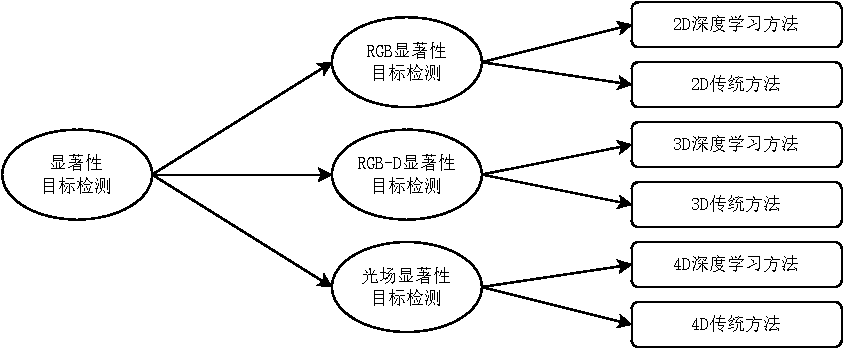
\includegraphics[width=0.90\linewidth]{figures/chapter1/kinds}
	\bicaption{显著性目标检测的分类}
	{Classification of salient object detection}  
	\label{chpt1:fig:kinds}
\end{figure}
%%%%%%%%%%%%%%%%%%%%%%%%%%%%%%%%%%%%%%%%%%%%%%%%%%%%%%%%%%%%%%%%%%%%%%%
\BiSubsection{RGB 显著性目标检测}{RGB Salient Object Detection}
\label{chpt1:title:rgb_methods}
%
%
当前,2D的显著性目标检测算法经历了传统算法和深度学习算法两个发展阶段。
传统的显著性目标检测算法,
属于从低层到高层的处理算法,
它们是一种刺激驱动的方式,
主要利用不同像素值的差异,主要体现在色彩对比度等方法;
和像素值区域的差异,主要体现在纹理、轮廓等先验线索来定位显著性目标所在的区域。
这些传统方法的优势在于快速和适应性强,
这些算法中常有基于对比度的先验假设,
基于中心先验假设和基于对象像素区域的先验假设三种。
对比度先验可分为局部对比度\upcite{itti1998model}和全局对比度方法\upcite{cheng2014global},
其中采用局部区域对比的检测方法,通过相邻像素的对比度,
或者综合考虑区域之间的像素对比度来辨别显著性物体。
这些方法在分析局部区域内的对比度差异时,可以有效地识别显著性目标,
因为显著性物体通常具有与周围环境不同的对比度特征。
相对于值考虑局部区域的像素贡献,
采用全局像素对比的方法以整个图像为单位,
探索整个图像不同区块之间的对比差异,
在一定程度上提高了显著性目标检测的定位能力。
中心先验是另一种常见的显著性检测先验,
它假设显著性物体往往位于图像的中心区域。
一些其他检测方法常用这些先验知识来辅助优化显著性预测图。
例如,Zhang等研究者\upcite{zhang2015minimum}
先通过全局像素对比的方式获取粗糙的显著性图,
再通过中心先验来对初始的显著性图进行细化处理,
提高了显著性目标的预测质量。
Jiang等学者\upcite{jiang2013salient}也采用类似的方式,
先通过区域对比的方式获得初始的显著性定位,
再根据各个区域的对象先验,
获取细粒度的特征,以此来优化每个区域的显著性图。
通过考虑显著性对象的形状、大小等特征,对象性先验可以有效地指导显著性目标的识别与定位,
进而提升检测性能。



%%%%%%%%%%%%%%%%%%%%%%%%%%%%%%%%%%%%%%%%%%%%%%%%%%%
%%
%% Split paragraphs
%%
%%%%%%%%%%%%%%%%%%%%%%%%%%%%%%%%%%%%%%%%%%%%%%%%%%%




以上提及的方法利用确定性先验知识,
再一些简单场景,即显著性前景和背景像素具有清晰差异时,
能够获得不错的检测效果。
然而,这些方法的鲁棒性较差,
在一些复杂场景,比如透明物体,带阴影物体或是傍晚等低光照场景下,
其检测效果非常不可靠。
相比之下,基于深度学习的检测算法,
能够通过学习带真值的数据集而理解不同的物理场景,
在一些困难场景也具有很高的检测精度。
近年来,基于编码器-解码器和特征聚合架构的显著对象检测
(SOD)
方法已取得了很高的性能
\upcite{gupta2020salient,mao2021generative,wang2021salient}。
MLMSNet\upcite{wu2019mutual}利用前景边界检测和边缘检测的监督。
AFNet\upcite{feng2019attentive}开发了一种关注反馈模块,以更好地探索目标结构。
EGNet\upcite{zhao2019egnet}利用关于显著边缘和显著对象的互补信息来提出边缘引导网络。
CPDNet\upcite{wu2019cascaded}提出了一个部分解码器,用于优化高级特征生成精确的显著性预测,在提升检测性能的同时显著提高了检测速度。
BASNet\upcite{qin2019basnet}通过顺序堆叠两个具有不同配置的
U-Net\upcite{1023770130.nh}实现了精细的预测模型。
AADFNet\upcite{zhu2019aggregating}设计了一个基于关注密集 ASPP 的网络,以选择性地使用小膨胀速率卷积和大膨胀速率卷积来获取局部和全局显著性信息。
GateNet\upcite{zhao2020suppress}设计了一个带有门控双分支结构,以建立不同级别特征之间的合作关系,以增加网络的可辨识性。
U2Net\upcite{qin2020u2}提出了一种新颖的 Residual U-block (RSU),可以在不降低特征映射分辨率的情况下获得内部多分辨率特征。
MINet\upcite{zhang2020multistage}提出通过采用多阶段的精化机制来增强前馈神经网络。
LDF\upcite{wei2020label}设计了一个双分支解码器,通过利用对象的主体和细节信息的互补性来预测显著性地图。
SAC\upcite{9094635}实施了一个空间衰减上下文模块来通过两轮递归转换传播和聚合显著特征。
CANet\upcite{ren2020salient}提出了一个具有上下文感知的注意力模块,通过同时建立每个像素与其周围全局和局部上下文的联系来检测显著区域。
%KRN\upcite{xu2021locate}在其粗定位模块中使用中间边缘监督。
ICON\upcite{zhuge2022salient}引入了三种不同的特征聚合、
完整性通道增强和部分-整体验证方法来进行显著性目标检测。
EDN\upcite{wu2022edn}使用极端下采样方法有效学习全局特征,并在解码器中应用尺度相关卷积构造金字塔结构 
%Scale-Correlated Pyramid Convolution 
来恢复本地细节。
这些方法的提出,提高了基于彩色图像的2D显著性目标检测的预测质量。




%当场景对比度低且模糊时,要识别显著对象的精细边界(或轮廓)仍然具有挑战性。在我们的工作中,我们从上述方法中获得灵感(例如,双分支解码器、ASPP、注意力和迭代精化),但我们的模型独特地应用了这些方法。



%%%%%%%%%%%%%%%%%%%%%%%%%%%%%%%%%%%%%%%%%%%%%%%%%%%%%%%%%%%%%%%%%%%%%%%
\BiSubsection{RGB-D 显著性目标检测}{RGB-D Salient Object Detection}
\label{chpt1:title:rgbd_methods}

%
%
%在RGB-D的显著性目标检测领域,深度图提供丰富的空间信息,这为在许多复杂场景下的显著性目标检测性能带来了显著提升。传统的RGB-D检测方法通常依赖形状、三维布局等低阶特征来定位显著性目标。
%Peng等学者\upcite{peng2014rgbd}提出了多阶段的检测模型,结合深度信息和图像信息进行显著性预测。
%Ren等研究者\upcite{ren2015exploiting}将RGB-D视为4通道数据来计算局部对比度,并将对比信息与全局先验知识相结合,提出了基于两阶段的显著性目标检测框架。一些RGB-D检测方法基于特定假设来定位显著性目标,比如认为靠近相机的目标更容易被识别为显著性目标。
%Feng等学者\upcite{shigematsu2017learning}根据这一假设,提出了一种局部背景封闭特征来识别显著性目标。这些方法证明了深度信息在显著性目标检测任务中的重要作用。然而,与传统RGB检测方法类似,这些方法存在泛化性较差的问题,当不满足先验知识或假设时,检测精度会明显下降。随着深度学习的进展,卷积神经网络能够提取深度图和RGB图像的高阶语义特征,从而大幅提升了RGB-D检测方法的性能水平。
%
%
%
%
%基于深度学习的 RGB-D 检测方法通常先提取RGB-D数据的特征,然后融合不同模态的特征来定位显著性目标,许多研究致力于研究更有效的跨模态特征融合方式。根据融合方式的不同,现有的基于深度学习的 RGB-D 方法可以大致分为前期融合、后期融合和多级融合三种方式。前期融合策略是指先融合多模态信息,然后提取特征来预测显著性,
%Qu等研究者\upcite{qu2017rgbd}遵循这种方式,将RGB图像和深度图同时输入深度网络进行显著性预测。后期融合策略则是先提取多模态信息特征,然后融合这些特征来预测显著性,
%Shigematsu等学者\upcite{shigematsu2017learning}采用后期融合方式,分别提取RGB图像和深度图的特征,然后将它们级联来定位显著性目标。与前述两种方式相比,多级特征融合在不同层级进行跨模态特征融合,使得不同层级的特征相互补充,在显著性目标检测任务中更为有效。
%Chen等研究者在PCA中\upcite{chen2018progressively}采用多级特征融合方式,引入跨模态互补感知融合模块,考虑RGB和深度图之间的联系,在特征融合时获取更充分和有效的信息。
%Piao等研究者\upcite{piao2019depth}提出了深度诱导的多尺度注意力网络,结合深度特征和RGB特征以不同尺度上下文信息融合,实现了精准的显著性定位。此外,研究者们还积极探索除特征融合外的RGB-D检测方法。
%在CPFP中,Zhao等学者\upcite{zhao2019contrast}利用增强的深度信息来增强显著性目标与背景之间的对比度,并将其与RGB特征级联以预测显著性。
%Chen等研究者\upcite{chen2019three}提出了一个自适应整合深度特征和RGB图像特征的注意力机制。




许多基于RGB-D 的显著性目标检测模型旨在通过探索有效的多模态相关性来提高显著性目标检测性能。
早期的工作侧重于用深度图增强RGB特征。
Piao等人\upcite{piao2019depth}提出了使用残差连接的深度细化块,将RGB和深度特征融合在一起。
Zhao等研究者\upcite{zhao2019contrast}通过将RGB特征与增强的深度图相乘来增强RGB特征的对比度。
Chen等人\upcite{chen2021rgb}提出了跨RGB和深度模态的预融合,
随后通过三维卷积进行深度特征融合。
现在,RGB-D 显著性目标检测方法提出了同时改进RGB特征和深度特征的复杂融合架构。
Wu等学者\upcite{wu2023hidanet}建议使用跨域监督和解码器融合的多尺度多级编码器融合方案,利用通道间的依赖关系。
Cong等人\upcite{cong2022cir}引入了渐进式注意力引导集成单元和重要性门控融合,
它在编码器和解码器阶段分别集成RGB和深度特征。
Zhang等研究者\upcite{zhang2021bts}提出了一个双向转移和选择模块,
以使RGB特征和深度信息在编码器阶段相互校正/改进。
尽管这些复杂的融合策略提高了RGB-D 显著性目标检测的性能,但也增加了模型的大小。




%%%%%%%%%%%%%%%%%%%%%%%%%%%%%%%%%%%%%%%%%%%%%%%%%%%
%%
%% Split paragraphs
%%
%%%%%%%%%%%%%%%%%%%%%%%%%%%%%%%%%%%%%%%%%%%%%%%%%%%




最近的研究表明,多尺度卷积神经网络(Convolutional Neural Network,CNN)在
%超分辨率\upcite{lai2017deep,dong2016accelerating}
%和图像去模糊\upcite{cho2021rethinking,kim2022mssnet}
超分辨率\upcite{lai2017deep}
和图像去模糊\upcite{cho2021rethinking}
方面可以比单尺度CNN取得更好的性能。
不同尺度的图像可以提供特定于比例的特征。如何有效地在不同尺度之间交换这些宝贵的信息是非常具有挑战性的。
作为一项多模态学习任务,
大多数现有的RGB-D显着性检测模型\upcite{peng2014rgbd,hu2022multi,cheng2014depth,zhao2020single,piao2020a2dele}侧重于有效的多模态特征融合,
这可以通过隐式多模态特征聚合或显式模态贡献评估来实现\upcite{zhang2021rgb,zhou2021specificity}。
考虑到深度可能存在噪声,一个主要方向是探索深度贡献\upcite{zhang2020select,wang2019adaptive},
旨在提炼更具信息量的深度特征,以实现有效的多模态学习。例如,
Ji等人\upcite{ji2021calibrated}提出了校准深度中潜在噪声的方法,
并引入了一个交叉参考模块,将校准后的深度与RGB特征融合。
Sun等研究者\upcite{sun2021deep}构建了深度分解模块,使用深度图的几何先验来过滤RGB图像中的噪声。
为了实现相同的目标,Zhang等人提出基于区域的特征备选策略,通过自监督学习,
实现能够更好地利用几何信息的辅助深度估计模块\upcite{zhang2021deep}。
%或改进模块\upcite{piao2021critical}。
除了确定性RGB-D显着性检测模型外,Zhang等学者\upcite{zhang2020uc}还探索了基于生成模型的显着性检测,
以解释显著性的“主观性质”。



%%%%%%%%%%%%%%%%%%%%%%%%%%%%%%%%%%%%%%%%%%%%%%%%%%%
%%
%% Split paragraphs
%%
%%%%%%%%%%%%%%%%%%%%%%%%%%%%%%%%%%%%%%%%%%%%%%%%%%%




%然而,在RGB-D显着性检测中使用多尺度CNN受到了所需的模型大小和计算量的限制。设计用于RGB-D SOD的多尺度CNN网络的主要挑战包括:1)模型大小。尽管处理多个尺度的图像,但设计的多尺度网络应具有适当的模型大小和快速推断速度;2)跨不同尺度的信息交换。




%%%%%%%%%%%%%%%%%%%%%%%%%%%%%%%%%%%%%%%%%%%%%%%%%%%%%%%%%%%%%%%%%%%%%%%%%%%%%%
\BiSubsection{光场显著性目标检测}{Light Field Salient Object Detection}
\label{chpt1:title:lf_methods}


在光场显著性目标检测领域,光场数据能够记录目标场景的空间信息并提供准确的深度信息,从而缓解困难场景下检测准确性受限的问题。光场数据记录了自然场景更全面、更完整的信息,对于显著性目标检测任务具有积极作用,因此越来越多关于利用光场数据提升检测性能的研究开始涌现。



%%%%%%%%%%%%%%%%%%%%%%%%%%%%%%%%%%%%%%%%%%%%%%%%%%%
%%
%% Split paragraphs
%%
%%%%%%%%%%%%%%%%%%%%%%%%%%%%%%%%%%%%%%%%%%%%%%%%%%%



光场显著性目标检测,也经历了从传统方法到可学习的深度卷积神经网络方法的转变。
传统方法通常采用手工制作的特征(例如,颜色对比度、纹理对比度和深度对比度)和先验(例如,位置先验、背景先验和边界连接先验)来检测显着对象。 
大多数方法采用先进行粗糙预测,然后在细化处理的多阶段检测方式,而且大部分研究都是基于光场焦点堆栈数据展开探索。
%
%
Li等人\upcite{li2014saliency}提出了第一个光场显着性数据集,并通过计算背景先验、位置先验和对比度线索来检测显着对象。
之后,Li等研究者\upcite{li2015weighted}提出了加权稀疏编码框架同时处理2D、3D和4D 显著性检测的问题,
收集非显著性区域来增强图像中其他显著的数据,
通过循环迭代来逐渐优化显著性目标的表示。
Zhang等人\upcite{zhang2015saliency}计算对比度显着图,
然后通过深度线索和彩色的像素线索之间的差异入手,
构建显著性图,
并以区域先验知识来强化预测。
Wang等学者\upcite{wang2017two}利用贝叶斯原理,
以概率的方式计算光场图像中的各种视觉特征。
Zhang等研究者\upcite{zhang2017saliency}
集成了从全焦点图像、深度图,散焦图片中提取不同语义信息表示,
尝试了随机搜索特征的方式。
最近,Piao 等研究者人\upcite{piao2019saliency}探索并
应用深度诱导的元胞感知机,
来构建进行显著性检测的子模块,汇总不同深度信息来进行最终的光场显著性目标检测。
传统的光场显著性检测方法,
存在预测质量差,易受干扰等缺陷,很难实现一个鲁棒性好的算法。
有关传统方法的更多详细信息可以在\upcite{fu2022light}中找到。


%%%%%%%%%%%%%%%%%%%%%%%%%%%%%%%%%%%%%%%%%%%%%%%%%%%
%%
%% Split paragraphs
%%
%%%%%%%%%%%%%%%%%%%%%%%%%%%%%%%%%%%%%%%%%%%%%%%%%%%



到了深度学习时代,几种深度学习方法对光场显著性目标检测的性能有显着提升。
由于不同的光场数据可视化形式,
基于深度学习的光场显著性目标检测方法也可以进行相应的划分。
有利用多视角图像和中心视角图像进行检测的深度学习方法,
也有使用全聚焦图和焦点堆栈进行检测的光场方法。



大多数基于深度卷积神经网络的光场显著性检测算法,
多利用全聚焦图和焦点堆栈构建双支路网络模型,
利用神经网络的非线性表示能力学习跨模态的信息提取,
来获取最终的显著性预测。
Piao等研究者\upcite{piao2019deep}首次使用深度卷积神经网络进行光场显著性目标检测。
在DFS\upcite{wang2019deep}中,Wang等研究者利用ConvLSTM\upcite{chen2015convolutional}
来处理焦点堆栈序列,该方法将焦点堆栈理解为序列输入,为每个序列单元生成权重矩阵,
用来加权每一张散焦图片特征并反馈到全聚焦支路特征上,
整体考虑了光场的数据特征来预测显著性目标预测。
Piao等团队\upcite{zhang2019memory}也使用了类似于循环神经网络的ConvLSTM来建模光场中焦点堆栈数据,
公布了当时主流的光场显著性目标检测数据集。
Liu等人\upcite{liu2021light}利用局部图网络来学习焦点堆栈特征,
通过循环优化,来逐步增强网络对显著性物体的感知。
Feng等研究者提出了NoiseLF\upcite{feng2022learning},
该方法首先通过传统方法构建噪声标签来进行无监督的光场显著性目标检测。
Wang等人提出了LFBCNet\upcite{wang2022lfbcnet},
构建了级联显著性检测支路和边缘预测支路的网络来进行光场显著性目标检测。




%在DLSD\upcite{piao2019deep}中,Piao等学者将光场显著性目标检测拆分为两个子任务:通过合成多视角图像来检测显著性对象。
%而Zhang等研究者\upcite{zhang2020light}在MAC中采用多视角图像阵列进行光场显著性目标检测,并建立了一个新的多视角图像阵列的数据集,通过对不同视角图像角度变化建模,将提取的特征输入至DeepLabV2\upcite{chen2017deeplab}的结构中以捕获多尺度信息。
%朴等人\upcite{piao2020exploit}提出了一种由焦点流和RGB流组成的不对称双流架构,以实现台式计算机和移动设备的多功能性。
%在LFNet\upcite{zhang2020lfnet}中,Zhang等人提出了细化模块和整合模块,通过整合模块融合光场特征,并利用细化模块进一步优化显著性预测值。
%在PANet\upcite{piao2021panet}中,Piao等研究者提出了一种区域级的探索光场数据方法,并提出了相应的特征整合策略,利用光场的全局信息来缓解大物体多目标检测不准确的问题。



%%%%%%%%%%%%%%%%%%%%%%%%%%%%%%%%%%%%%%%%%%%%%%%%%%%
%%
%% Split paragraphs
%%
%%%%%%%%%%%%%%%%%%%%%%%%%%%%%%%%%%%%%%%%%%%%%%%%%%%

尽管大多数方法输入全焦点图像和焦点堆栈,但一些方法\upcite{jing2021occlusion, wang2022lfbcnet, zhang2022exploring}提出使用多视图和中心视图图像来检测显着对象。 
%另一方面,利用多视角图像进行显著性检测的深度学习模型
这些方法致力于从不同视角间挖掘有效特征之间的关联。
Zhang等人\upcite{zhang2020light}提出了一种深度网络,通过利用微透镜图像中丰富的角度信息来检测显着物体。 
Zhang等学者\upcite{zhang2021geometry}提出了一种图神经网络,通过有效探索多视图图像之间的空间和视差相关性来预测显着图。 
Jing等人\upcite{jing2021occlusion}提出了一种遮挡感知网络,
从极平面图像(Epipolar Plane Images,EPI)中提取遮挡边界特征以进行显着性检测。 
Zhang等人\upcite{zhang2022exploring}提出了一种光场合成网络来产生可靠的4D信息并驱动显着性检测。 
然而,上述方法的性能不如基于焦点堆栈输入的光场方法。 
这些使用多视角图像作为输入的方法集成了解码器中整个图像矩阵的特征,
忽略了不同视角对检测的相对贡献,并且容易受到非显着背景的影响。 


%%%%%%%%%%%%%%%%%%%%%%%%%%%%%%%%%%%%%%%%%%%%%%%%%%%
%%
%% Split paragraphs
%%
%%%%%%%%%%%%%%%%%%%%%%%%%%%%%%%%%%%%%%%%%%%%%%%%%%%


除了基于卷积神经的显著性检测方法外,
基于 Transformer 的显著性检测方法也开始崭露头角,
有应用于 
RGB 显著性目标检测\upcite{liu2021visual, siris2021scene}和 
RGBD 显著性目标检测\upcite{liu2021tritransnet, wang2021mutualformer}
和光场显著性目标检测\upcite{liu2023lftransnet}。
Transformer 首先由 Vaswani 等人提出\upcite{vaswani2017attention},
已广泛应用于自然语言处理
(NLP)
。
ViT (Vision Transformer)由 Dosovitskiy 等人提出\upcite{dosovitskiy2020image},
首先将Transformer应用于图像域。
相比具有局部感受野的深度卷积神经网络,
Transformer由于其强大的全局信息捕获能力,
基于Transformer架构的网络在不同视角任务上表现出了优异的性能。
最近的工作探索了将 Transformer 应用于各种视觉任务:
图像分类\upcite{chen2020generative, dosovitskiy2020image}、
目标检测\upcite{zhu2020deformable, dai2021up, sun2021rethinking}、
语义分割\upcite{chen2021pre, wang2021end}、
图像增强\upcite{yang2020learning, chen2021pre}、
图像生成\upcite{parmar2018image}和 
视频处理\upcite{zhou2018end, zheng2020end}等,
用以缓解卷积神经网络有限的全局信息学习能力。



研究者探索了将Transformer架构应用于显著性目标检测任务,如
Liu等人\upcite{liu2021visual}设计了一个基于纯Transformer架构的统一模型,通过建模远程依赖性来预测显着性。
刘等人\upcite{liu2021tritransnet}提出了一种用于 RGB-D 显着目标检测的三元组变换器嵌入模块,通过学习跨层的远程依赖关系来增强高级特征。 
Siris等人\upcite{siris2021scene}提出了一种上下文实例转换器来捕获对象和场景上下文之间的上下文关系,以实现更准确的显着性推断。 
Wang等人\upcite{wang2021mutualformer}提出了一种基于Transformer的多模态融合模块来增强和融合RGB和深度图像特征。
受益于Transformer的使用,这些方法可以获得更准确的场景上下文特征,并在复杂场景中表现出更好的检测性能。 然而,如何将Transformer应用于光场显著性目标检测领域,
发挥Transformer架构在建立常成依赖方面的优势,
尚未得到全面探讨。 






%%%%%%%%%%%%%%%%%%%%%%%%%%%%%%%%%%%%%%%%%%%%%%%%%%%%%%%%%%%%%%%%%%%%%%%
\BiSubsection{现存挑战}{Challenges}


%%%%%%%%%%%%%%%%%%%%%%%%%%%%%%%%%%%%%%%%%%%%%%%%%%%
%%
%% Split paragraphs
%%
%%%%%%%%%%%%%%%%%%%%%%%%%%%%%%%%%%%%%%%%%%%%%%%%%%%



随着十年多以来,机器学习和人工智能的发展,
基于深度卷积神经网络构建的光场显著性目标检测算法,
可以提取光场可视化表示中的显著语义特征,
提升了显著性目标检测的算法性能。
但是由于光场的高维数据表示,
怎么使用深度神经网络在繁杂的光场信息中
找出相似的像素物体,及不同视角之间的像素差异,
并从中决策出显著性的区域表示,依然有很大难度。
如果所有隐含于光场的显著性信息都需要深度神经网络自主取学习,
这需要网络具有极高的数据吞吐量,
并且依赖大量的有监督学习样本来进行训练。
一般情况下,训练样本越多,模型的泛化能力就越好。
但是现实中,可用光场数据是有限的,
具有像素级密集标注的光场显著性目标检测数据集更为稀少。
难以只依赖超大量的数据量来拟合性能足够的光场显著性检测网络。
所以,依赖光场数据内部之间的关联来构建光场显著性目标检测算法,
是现有深度神经网络的普遍做法。
如何设计网络模型来有效的提取光场数据中隐含表示,
以及如何融合全聚焦图和焦点堆栈两个支路的特征,
是每一个光场显著性检测领域研究者需要考虑的问题。



%%%%%%%%%%%%%%%%%%%%%%%%%%%%%%%%%%%%%%%%%%%%%%%%%%%
%%
%% Split paragraphs
%%
%%%%%%%%%%%%%%%%%%%%%%%%%%%%%%%%%%%%%%%%%%%%%%%%%%%

%如何有效利用有限的光场数据来设计网络模型,


对于前一个问题,最近的光场方法有利用3D卷积神经网络来处理高维的焦点堆栈信息,
虽然能够在一定程度上提取焦点堆栈的高级语义信息,但也带来了巨大的参数量和计算量。同时这种依靠网络大吞吐量的学习方法,无法建模焦点堆栈的聚焦差异,
这限制了光场信息的发挥。
也有将光场焦点堆栈转换为序列问题来处理,依靠序列建模,如ConvLSTM等来进行显著性表达建模,这种方法虽然能够考虑不同切片之间的差异,但是存在序列信息遗忘的问题,
使得网络更加关注焦点切片序列中部分信息,无法以进行光场数据的整体建模。



对于后一个问题,现有方法多利用通道的拼接来融合两个模态的信息,
两个模态的差异提取依赖卷积核的权重累计,
无法显示提取相似信息与互补的差异信息。
也有通过平均池化等策略来生成通道注意权重,特征和注意权重在通道维度相乘来融合高维焦点堆栈数据的方法,
其生成通道权重时只依赖自身模态的整体信息,忽略了引入跨模态的互补信息,
同样限制了网络建模光场信息。



%最近的光场显著性目标检测算法通常会引入多尺度特征图,
%并在多尺度特征图上应用全局注意力机制,
%侧重对焦点切片内部与显著性物体相似的特征的强化,
%网络并不能很好捕获不同散焦切片之间的聚焦差异,
%使得网络只能感知有限的光场数据信息。




%%%%%%%%%%%%%%%%%%%%%%%%%%%%%%%%%%%%%%%%%%%%%%%%%%%
%%
%% Split paragraphs
%%
%%%%%%%%%%%%%%%%%%%%%%%%%%%%%%%%%%%%%%%%%%%%%%%%%%%



应对以上两个构建光场显著性检测模型的难点,
构建能够提取光场切片级信息的检测网络,
差异化融合两个模态的信息,构建高效可用的光场显著性目标检测网络,
还需要进一步的探索和研究。


%
%本文探索了两种不同的聚焦感知方法。
%对与最大化提取和利用光场数据中隐含的有效场景信息,
%本文构建焦点感知网络,通过利用可学习参数在光场整体输入上,
%学习焦点堆栈和全聚焦图的切片级焦点相关向量,
%并传递不同切片之间的聚焦差异信息。
%并交互融合光场两个模态的互不信息,
%促进深度神经网络能够精确感知场景中的显著性物体表示。
%\todo 



%%%%%%%%%%%%%%%%%%%%%%%%%%%%%%%%%%%%%%%%%%%%%%%%%%%%%%%%%%%%%%%%%%%%%%%%%%%%%%%%%%%%%
\BiSection{论文主要内容及结构安排}{Main Content and Structural Arrangement}

\BiSubsection{主要内容}{Main Content}
%
%本篇文章以显著性目标检测为核心内容,着眼于探索受限数据驱动的光场显著性检测方法。研究从两个方面入手,一是设计能有效利用有限光场数据的网络模型,二是构建有效增强光场数据的算法,以缓解数据稀缺的挑战。在关于如何设计适用于有限光场数据的深度检测网络模型方面,本文提出了一种新的区域感知网络。这个网络与目前方法中使用的全局注意力不同,它从局部角度出发,考虑了每个焦点切片中不同区域对显著性预测的作用,更充分地利用了有限的光场数据。多源学习模块结合显著性、边界和中心位置信息生成特征整合策略,针对焦点堆栈的特征进行区域级整合,聚焦性识别模块考虑多聚焦特性对显著性的影响,并更新整合策略以更好地突出显著性区域并抑制非显著性区域。
%
%另一方面,关于如何设计有效增强光场数据的算法,本文提出了一种基于数据增强的光场显著性目标检测方法。相对于传统的数据增强方法,该方法引入了几何增强模块,通过结合图像修复网络和空间变换网络重新组合场景中的显著对象和背景,以尽可能扩增当前的光场数据集。聚焦性补偿模块则利用风格迁移网络进一步优化组合图像中焦点堆栈的真实性。此外,该方法还提出了一个不确定性学习策略,用于联合训练合成数据和真实数据,通过不同对待质量的合成数据,减小合成数据对网络训练的不利影响。



显著性目标检测的目标在于识别图像场景中最吸引人眼注意的像素或区域,
是计算机视觉领域中一个重要的基础任务。
现有的显著性目标检测方法,多依赖其处理的数据形式进行分类,
分别包含RGB、RGB-D和光场方法三种。
与输入彩色图像的RGB数据和辅以深度图像的RGB-D数据相比,光场数据包含了更丰富的场景信息,可以满足建模复杂场景信息的需求。
近几年来,
随着机器学习和人工智能领域的发展,
基于可学习卷积神经网络的算法,
逐渐超越了传统基于先验等手工特征的处理方法,
将光场显著性目标检测性能提升到了一个新的阶段。
%
%
%然而,实际应用中存在较高的光场数据获取成本、复杂的光场多线索信息处理以及耗时耗力的显著性像素级标注,这导致当前光场显著性目标检测数据稀缺,为深度模型提供足够支持的数据不足。为解决这些问题,本文从高效利用光场信息和增广光场数据两个角度出发,探索利用有限数据驱动的光场显著性目标检测方法。
%
%
%复杂的光场信息提取以及跨模态的光场信息融合难等问题,
%
%
然而,实际应用中存在如何有效提取和利用光场复杂数据中隐含的有效场景信息,
以及如何提取跨模态互补信息表示并进行两个模态信息融合等问题。
导致了当前光场显著性检测深度模型难以有效辨别光场场景的的显著性物体表示。
%
%
为了解决这些问题,本文从焦点感知和视角增强两个角度出发,
探索基于聚焦感知的光场显著性检测方法。
本文的两个主要工作及创新点如下所述:









%%%%%%%%%%%%%%%%%%%%%%%%%%%%%%%%%%%%%%%%%%%%%
%
% 第一个工作点
%
%%%%%%%%%%%%%%%%%%%%%%%%%%%%%%%%%%%%%%%%%%%%%

%其中令牌通信模块通过可学习的嵌入式令牌汇总建立全聚焦图片和焦点堆栈的切片级特征
%


(1)
%
%
面对如何有效利用复杂场景中丰富的光场线索的挑战,
本文提出了一种焦点感知网络探索光场数据的方法。
%
%
该方法主要包含两个部分:令牌通信模块和焦点感知增强策略。
%
%
为了汇总全聚焦图片和焦点堆栈的切片级特征,
本文提出了使用可学习的嵌入式令牌,
通过对每个图像划分图像块,并在每个图像块上附加嵌入式令牌,
送入注意力机制进行计算,从而汇总每张图片的语义信息,
为了跨切片的信息交互,使用嵌入式令牌作为信息传递的桥梁,
促进网络对空间上下文建模。
%
%
为了充分考虑不同散焦切片对于显著性的影响,并进行跨模态的信息融合,
提出焦点感知增强策略,通过判断每个散焦切片的聚焦程度,
来突出不同焦点切片中显著性区域,
同时抑制非显著性区域带来的负面影响。
%
%
相比现有的方法,本文方法通过附加可学习嵌入式令牌的方式,
对光场的整体三维场景进行了切片级的探索,
并考虑了不同散焦切片对显著性预测的贡献,
能够更有效的利用光场信息。







%%%%%%%%%%%%%%%%%%%%%%%%%%%%%%%%%%%%%%%%%%%%%
%
% 第二个工作点
%
%%%%%%%%%%%%%%%%%%%%%%%%%%%%%%%%%%%%%%%%%%%%%
(2)
%
%
面对如何高效的利用光场数据中全聚焦图和焦点堆栈两个模态的差异信息,
本文提出了一种基于视角增强的网络来探索光场数据的方法。
%
%
该方法主要包含两个主要部分:视角增强注意力模块和感知对比学习策略。
%
%
为了强化两个模态的信息表示,提出视角增强注意力模块,
引入跨模态的交叉注意力计算来学习互补信息,
并在对两个模态做交叉注意力时引入跨模态的掩码表达,
进一步加强注意力权重在不同聚焦区域上的显著性表达。
%
%
为了进一步增强网络对于显著性物体的辨识能力,
提出感知对比学习策略,
使网络能够考虑显著性预测的前景区域内部、与背景区域内部的一致性表达。
%
%
相比现有的光场显著性检测方法,本文方法对光场数据进行跨模态的特征融合,
充分考虑了焦点堆栈和全聚焦图对最终显著性预测的贡献,
能够产生更为鲁棒的显著性物体表达。



%%%%%%%%%%%%%%%%%%%%%%%%%%%%%%%%%%%%%%%%%%%%%%%%%%%%%%%%%%%%%%%%%%%%%%%%%%%%%%%%%%%%%
\BiSubsection{结构安排}{Structural Arrangement}



第一章先介绍了光场显著性目标检测的研究背景和意义,
再阐述了目前显著性目标检测领域的研究工作进展,
分析了目前光场显著性目标检测方法中存在的挑战。



第二章,介绍在光场显著性检测任务重使用到的相关理论及方法。
主要包括光场技术的基本成像原理、光场数据不同的可视化表示方式、
基于多视角图像的光场显著性目标检测原理和
基于焦点堆栈的光场显著性目标检测原理,
并介绍了显著性目标检测中用于评估模型性能的评价指标。


第三章详细介绍了基于焦点感知的光场显著性目标检测方法。
首先分析了现有光场显著性目标检测方法存在的问题,并阐述了研究的动机。
随后介绍了所提出的网络模型结构,
以及涉及到的令牌交互模块和焦点感知增强策略的具体应用方法。
最后,展示了实验设置和结果分析,证明了所提出方法的卓越性能。


在第四章中,详细阐述了基于视角增强的光场显著性目标检测方法。
探讨分析了现有光场方法中注意力机制的应用与不足,并阐述本文研究动机,
详细介绍了视角增强注意力机制的框架结构
和感知对比学习策略的具体实施方法。
最后,呈现了实验设置和结果分析,以验证所提出方法的显著优势。































